\documentclass[journal, a4paper]{IEEEtran}

% some very useful LaTeX packages include:

%\usepackage{cite}      % Written by Donald Arseneau
                        % V1.6 and later of IEEEtran pre-defines the format
                        % of the cite.sty package \cite{} output to follow
                        % that of IEEE. Loading the cite package will
                        % result in citation numbers being automatically
                        % sorted and properly "ranged". i.e.,
                        % [1], [9], [2], [7], [5], [6]
                        % (without using cite.sty)
                        % will become:
                        % [1], [2], [5]--[7], [9] (using cite.sty)
                        % cite.sty's \cite will automatically add leading
                        % space, if needed. Use cite.sty's noadjust option
                        % (cite.sty V3.8 and later) if you want to turn this
                        % off. cite.sty is already installed on most LaTeX
                        % systems. The latest version can be obtained at:
                        % http://www.ctan.org/tex-archive/macros/latex/contrib/supported/cite/

\usepackage{graphicx}   % Written by David Carlisle and Sebastian Rahtz
                        % Required if you want graphics, photos, etc.
                        % graphicx.sty is already installed on most LaTeX
                        % systems. The latest version and documentation can
                        % be obtained at:
                        % http://www.ctan.org/tex-archive/macros/latex/required/graphics/
\usepackage{subfig}
                        % Another good source of documentation is "Using
                        % Imported Graphics in LaTeX2e" by Keith Reckdahl
                        % which can be found as esplatex.ps and epslatex.pdf
                        % at: http://www.ctan.org/tex-archive/info/

%\usepackage{psfrag}    % Written by Craig Barratt, Michael C. Grant,
                        % and David Carlisle
                        % This package allows you to substitute LaTeX
                        % commands for text in imported EPS graphic files.
                        % In this way, LaTeX symbols can be placed into
                        % graphics that have been generated by other
                        % applications. You must use latex->dvips->ps2pdf
                        % workflow (not direct pdf output from pdflatex) if
                        % you wish to use this capability because it works
                        % via some PostScript tricks. Alternatively, the
                        % graphics could be processed as separate files via
                        % psfrag and dvips, then converted to PDF for
                        % inclusion in the main file which uses pdflatex.
                        % Docs are in "The PSfrag System" by Michael C. Grant
                        % and David Carlisle. There is also some information
                        % about using psfrag in "Using Imported Graphics in
                        % LaTeX2e" by Keith Reckdahl which documents the
                        % graphicx package (see above). The psfrag package
                        % and documentation can be obtained at:
                        % http://www.ctan.org/tex-archive/macros/latex/contrib/supported/psfrag/

%\usepackage{subfigure} % Written by Steven Douglas Cochran
                        % This package makes it easy to put subfigures
                        % in your figures. i.e., "figure 1a and 1b"
                        % Docs are in "Using Imported Graphics in LaTeX2e"
                        % by Keith Reckdahl which also documents the graphicx
                        % package (see above). subfigure.sty is already
                        % installed on most LaTeX systems. The latest version
                        % and documentation can be obtained at:
                        % http://www.ctan.org/tex-archive/macros/latex/contrib/supported/subfigure/

\usepackage{url}        % Written by Donald Arseneau
                        % Provides better support for handling and breaking
                        % URLs. url.sty is already installed on most LaTeX
                        % systems. The latest version can be obtained at:
                        % http://www.ctan.org/tex-archive/macros/latex/contrib/other/misc/
                        % Read the url.sty source comments for usage information.

%\usepackage{stfloats}  % Written by Sigitas Tolusis
                        % Gives LaTeX2e the ability to do double column
                        % floats at the bottom of the page as well as the top.
                        % (e.g., "\begin{figure*}[!b]" is not normally
                        % possible in LaTeX2e). This is an invasive package
                        % which rewrites many portions of the LaTeX2e output
                        % routines. It may not work with other packages that
                        % modify the LaTeX2e output routine and/or with other
                        % versions of LaTeX. The latest version and
                        % documentation can be obtained at:
                        % http://www.ctan.org/tex-archive/macros/latex/contrib/supported/sttools/
                        % Documentation is contained in the stfloats.sty
                        % comments as well as in the presfull.pdf file.
                        % Do not use the stfloats baselinefloat ability as
                        % IEEE does not allow \baselineskip to stretch.
                        % Authors submitting work to the IEEE should note
                        % that IEEE rarely uses double column equations and
                        % that authors should try to avoid such use.
                        % Do not be tempted to use the cuted.sty or
                        % midfloat.sty package (by the same author) as IEEE
                        % does not format its papers in such ways.

\usepackage{amsmath}    % From the American Mathematical Society
                        % A popular package that provides many helpful commands
                        % for dealing with mathematics. Note that the AMSmath
                        % package sets \interdisplaylinepenalty to 10000 thus
                        % preventing page breaks from occurring within multiline
                        % equations. Use:
%\interdisplaylinepenalty=2500
                        % after loading amsmath to restore such page breaks
                        % as IEEEtran.cls normally does. amsmath.sty is already
                        % installed on most LaTeX systems. The latest version
                        % and documentation can be obtained at:
                        % http://www.ctan.org/tex-archive/macros/latex/required/amslatex/math/



% Other popular packages for formatting tables and equations include:

%\usepackage{array}
% Frank Mittelbach's and David Carlisle's array.sty which improves the
% LaTeX2e array and tabular environments to provide better appearances and
% additional user controls. array.sty is already installed on most systems.
% The latest version and documentation can be obtained at:
% http://www.ctan.org/tex-archive/macros/latex/required/tools/

% V1.6 of IEEEtran contains the IEEEeqnarray family of commands that can
% be used to generate multiline equations as well as matrices, tables, etc.

% Also of notable interest:
% Scott Pakin's eqparbox package for creating (automatically sized) equal
% width boxes. Available:
% http://www.ctan.org/tex-archive/macros/latex/contrib/supported/eqparbox/

% *** Do not adjust lengths that control margins, column widths, etc. ***
% *** Do not use packages that alter fonts (such as pslatex).         ***
% There should be no need to do such things with IEEEtran.cls V1.6 and later.

%Start: Das hier sorgt dafür, dass Umlaute funktionieren.
%\usepackage[main=ngerman, english]{babel}
\usepackage[main=ngerman, english]{babel}
\usepackage[utf8]{inputenc}
\usepackage{algorithm}
\usepackage{algorithmic}
\usepackage{amsmath}
\usepackage{gensymb}
%Ende: Das hier sorgt dafür, dass Umlaute funktionieren.

% Your document starts here!
\begin{document}
\selectlanguage{english}
% Define document title and author
	\title{Waddington's epigentic landscape}
	\author{Felicia Burtscher, Thomas Hadler, Hanna Wulkow 
	\thanks{}}
	\markboth{FU Berlin: Mathematical aspects in machine learning -- Summer Semester 2017}{}
	\maketitle

% Write abstract here
\begin{abstract}
In this project, a data set of Simpsons character pictures was used to test the validity of a random forest implementation. Decision trees are a machine learning method based on the idea of human decision making. Random forest are an expansion of that. The pictures from the data set were preprocessed using hog features.
The resulting random forests were created using a training set and validated using a smaller test set. The results were outstandingly good: even for small random forests well more than 50\% of the characters could be classified correctly. 
\end{abstract}
%\tableofcontents 
% Each section begins with a \section{title} command
\section{Task Description}

Our data set consists of images of 20 characters of \textit{The Simpsons} with labels. The data originates from the Kaggle contest \textit{Simpsons by the Data}. There are 200 to 1500 examples per character offering an unbalanced data set. The images have different shapes and the characters are scattered throughout the images. Our goal is to develop an algorithm which given an input image containing a Simpson character is capable to classify, i.e. recognize the Simpsons character in the image correctly. In \textit{The Simpsons} data set this is the character the image shows. We are looking for a function that maps the input images to the labels of the images.
\begin{figure}[!ht]
	\centering
  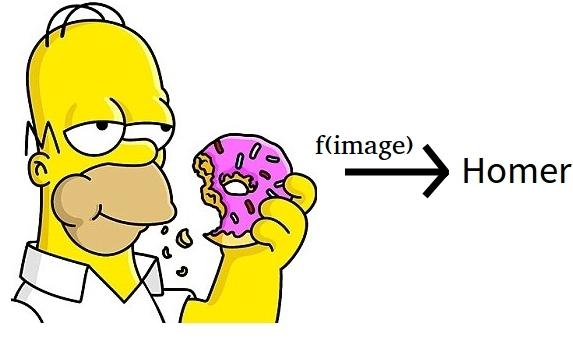
\includegraphics[width=0.3\textwidth]{Image3.jpeg}
	\caption{Homer Simpson}
	\label{Homer}
\end{figure}

\section{Mathematical Description of Images}
We work with images as input to our classification algorithm. Thus we describe the nature of our input here first.
Images are represented as tensors of rgb values. \textit{The Simpsons} data set consists of images of approximately \( 110 \times 110 \) pixels, each with three values in \{0, ..., 255\} representing the red, green and blue intensity of the specific pixel. This means that each image can be mapped to a 36300 dimensional vector with values in \{0, ..., 255\}. 
These vast dimensions illustrate the difficulty of this problem and show that it is not trivially solvable. We have \( 256^{36300}\) different possible vectors. 
Estimating a vector in a 36 300 dimensional vector space would be hard enough, estimating a vector of this dimension with only a couple thousand examples makes this practically impossible without exploiting additional information.

\section{Preprocessing the Data}

We use several preprocessing steps to transform the images to useful input data. The first step deals with the rescaling of the images to same shapes. The second step reduces the dimensionality of the problem by exploiting features. The resulting feature image is then the input to the algorithm.
\newline

\subsection{Rescaling the Data}
As mentioned in the paragraph before, initially the images come in different shapes. The width is between 70 and 170 pixels, the height is between 80 and 180 pixels. Since the classification algorithm takes a fixed number of input values, the images must be transformed into the same shape. 
\begin{figure}[!ht]
	\centering
  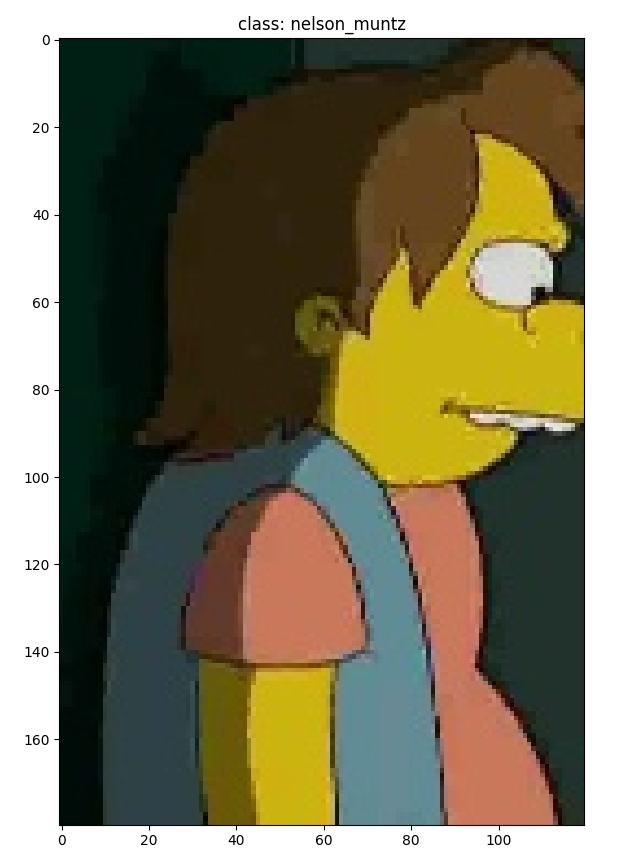
\includegraphics[width=0.2\textwidth]{Image4.png}
  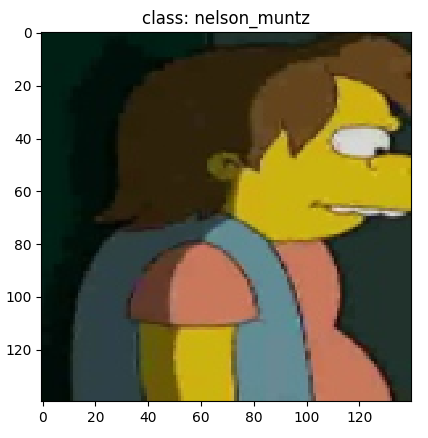
\includegraphics[width=0.2\textwidth]{Image5.png}
	\caption{Unscaled Nelson (left), Scaled Nelson (right). Best viewed on a monitor.}
	\label{fig7}
\end{figure}

We took the simplest route to achieving this and used bilinear interpolation to scale all images to the shape \( 110 \times 110 \) with three rgb values each. This then results in the 36300 values mentioned before.

\subsection{Features}
This section elaborates on features in general first. Then we move on to Histograms of Oriented Gradients (HOG), a feature descriptor developed by Dalal and Triggs in 2005 for human detection in images. We use this algorithm to create the feature inputs for our classifier.

\subsubsection{Definition}
A feature is a piece of information which is relevant for solving the computational task at hand. The idea of a feature is to reduce the vast amount of information given with the data to the relevant information within it. The assumption of a feature is that a large amount of the given information is essentially redundant or inconveniently expressed and can be reduced to a far more compact representation without losing a large amount of the overall information. This compact representation is called a feature.

\subsubsection{Computer Vision Features}
When working with images, video, ct-scans, etc. a computer vision specific dependency begins to take the spotlight. Pixels that lie close together tend to interact more strongly than pixels far apart. Within an image the pixel in the bottom left corner and the top right corner have little to do with each other. But pixels within a region can form larger features like corners, circles, noses, mouths or a fur-like texture. This locality- or neighborhood-characteristic is what is commonly used to create features in computer vision problems.

\subsubsection{Histogram of Oriented Gradients}
We recommend reading the original HOG-paper since it is very thorough and the exact execution of steps would be hard to elaborate on here. The procedure for creating the HOG-image from the original is roughly as follows:\newline
1) Compute the gradients\newline
2) Weighted vote into spatial and orientation bins\newline
3) Contrast normalize over overlapping spatial blocks\newline

\textbf{Compute the gradients}\newline
Dalal and Triggs tested several derivative masks but the simple mask $(-1,0,1)$ for x-direction and $(-1,0,1)^T$ for y-direction proved to be best. This mask is applied to every pixel's colors.
\newline

\textbf{Weighted vote into spatial and orientation bins}\newline
Now histograms of oriented gradients are created. To do this, the image is divided into cells of \( n \times n \) pixels. For each cell, a bin is created with a certain number of orientations. Every orientation spans a certain range of gradient direction. For example, four bins could mean that bin one collects all gradients within the cell that have an angle between 0\degree and 90\degree. Every gradient is now interpolated between the closest orientations and between the closest cells it belongs to.\newline

\textbf{Contrast normalize over overlapping spatial blocks}\newline
Instead of simply using these pooled interpolated gradients as inputs to the classifier the histograms are normalized several times with their neighboring cells and concatenated to a vector for each cell.

\begin{figure}[!ht]
	\centering
  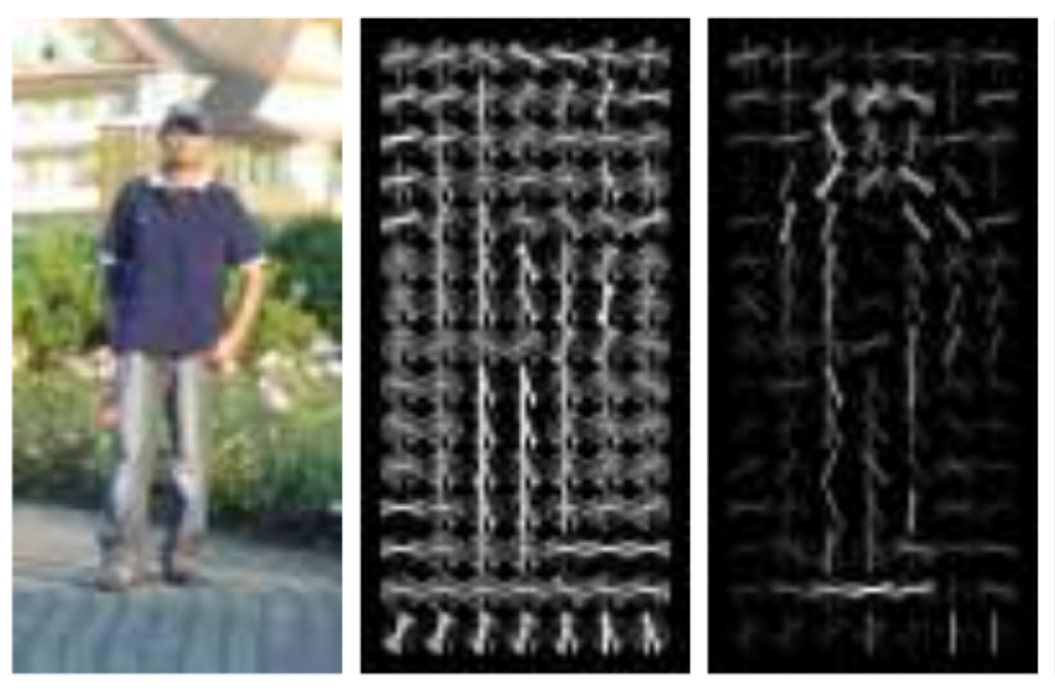
\includegraphics[width=0.4\textwidth]{Image2.png}
	\caption{Visualization of HOG feature-image. Extracted from [3]. Best viewed on a monitor.}
	\label{hog}
\end{figure}

% Main Part
\section{Methods}
% You can insert a line break manually with two backslashes, if needed: \\
The main algorithm we use is \textit{Random Forest} which is an adaptation of decision trees.

\subsection{Decision Trees}

Decision trees are built by a \textit{greedy} algorithm. 
The algorithm searches through each independent variable (here attributes) to find a value of a single variable that best splits the data into two (or more) groups. Typically, the best split minimizes the impurity of the outcome in the resulting data subsets. For these two resulting groups, the process is repeated until a stopping criterion applies.  \\
Decision trees are easy to understand and interpret and robust to noisy data. However, using information gain they are biased in favor of those attributes that give lots of subsets. Also, calculations can get very complex, particularly if many values are uncertain. At the same time they often suffer from high variance, i.e. they tend to overfit. A decision tree keeps splitting up the data until it ends up with pure sets, so it will always classify the training example perfectly. As the tree gets bigger and bigger, it becomes more accurate on the training data but at some point it will become less accurate on future test data, that is data we have not seen before. For a bias-variance trade-off we want to introduce randomization: we combine the prediction of several randomized trees into a single model.

\begin{figure}[!ht]
	\centering
  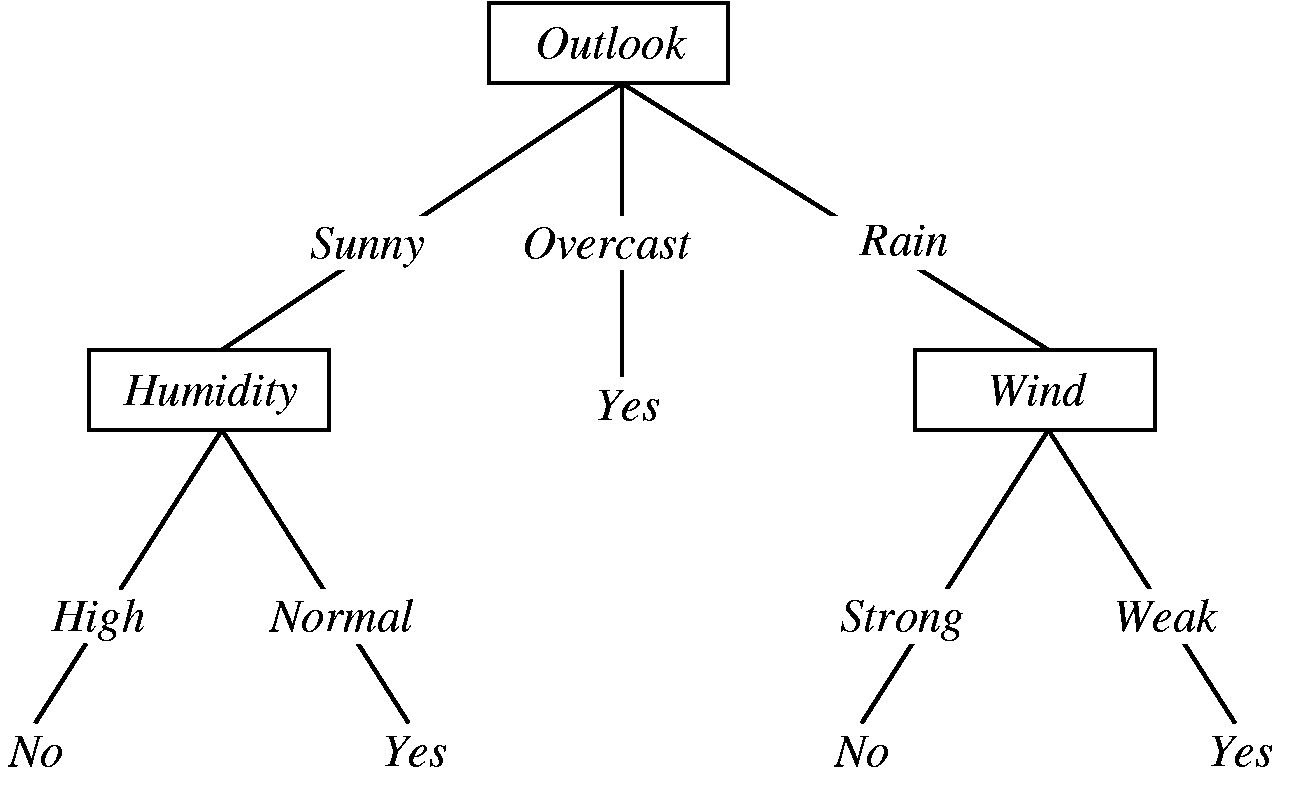
\includegraphics[width=0.4\textwidth]{ID3.png}
	\caption{Example of a decision tree from \cite{decisiontree}}
	\label{decisiontree}
\end{figure}

\subsection{Random Forest}

Instead of growing a single tree, Random Forest grows a large number of different decision trees. There are two main differences to the construction of decision trees: First, from the set of training data \( D \) we choose a random sample \( D_{i} \). Second, at each node we choose a random subset of features, \( S \), and only consider splitting on those features. Each tree is fully grown and not pruned. \\ 
Using majority vote, the decision tree then finds the joint set of variables that produce the strongest classification model. \\
Random Forest is one of the most robust and effective machine learning algorithms for many problems. \\

We use the C4.5 algorithm that uses information gain as the splitting criterion. Growing the decision tree from the root down, it greedily selects the next best attribute using information gain and then recursively calls the algorithm on its child nodes. The growing stops when all instances belong to a single value of target feature -- we call this a "pure" subset -- or when the best information gain is not greater than zero or any other stopping criteria defined such as tree depth. \\ It does not apply any pruning procedures nor does it handle numeric attributes or missing values. The following pseudo code taken from \cite{pseudocode} explains the algorithm.
%\begin{figure}
\begin{algorithm}
\caption{C4.5(D)}
\begin{algorithmic}
\REQUIRE an attribute-values data set D
\STATE{$\text{Tree}$ = $\{ \}$}
\IF{$D$ is "pure" OR other stopping criteria met}
\STATE terminate
\ENDIF
\FORALL{attribute a $\in D$} 
\STATE{Compute information-theoretic criteria if we split on $a$} 
\ENDFOR
\STATE{$a_{best} = $ Best attribute according to above computed criteria}
\STATE{Tree $=$ Create a decision node that tests $a_{best}$ in the root}
\STATE{$D_{v} =  $ Induced sub-data sets from $D$ based on $a_{best}$}
\FORALL{$D_{v}$} 
\STATE{$\text{Tree}_{v}$ = C4.5($D_{v}$)}
\STATE{Attach $\text{Tree}_{v}$ to the corresponding branch of Tree}
\ENDFOR
\RETURN Tree
\end{algorithmic}
\end{algorithm}
%\end{figure}

The idea of decision trees is rather simple; the question that is not so trivial is: How to select the best attribute?

\subsection{Information Gain}
For the sake of of simplicity, assume we have a binary decision problem. Our hypothesis is "Homer Simpson is in the picture". We therefore have positive examples (i.e. supporting our hypothesis) and negative examples in our subset \( S \). Our goal is to get items in pure sets, that is either only positive or only negative examples. This explains why a simple posterior probability computation falls short as it is not symmetric and \textit{all negative} is as pure as \textit{all positive}. As an alternative we can use entropy from information theory.

\subsubsection{Entropy}
Entropy measures the uncertainty of a class in a subset of examples \( S \). It is defined by
\[ H(S) = -p_{+} \cdot log_{2} p_{+} -p_{-} \cdot log_{2} p_{-}   \] where \( S \) is the subset of training examples and \( p_{+} \) and \( -p_{-} \) are the positive and negative examples in \( S \). \\ In our multi-class classification problem ("What character is seen on the picture?") this equation generalizes to 
\[ H(S) = - \sum_{i=1}^{n} p_{i} \cdot log_{2} p_{i}.  \]
We can interpret the entropy as follows: What is the amount of bits we need to convey, i.e. how many bits do we need to spend to tell if \( x \) is positive or negative assuming that it belongs to \( X \)? As a result, entropy tells us how pure (entirely "negative" or "positive") or impure one subset is. For instance, if a subset is pure, we have 0 bits whereas if it is (fully) impure (say 50\% positive, 50\% negative) we need 1 bit to be certain.\\
In general, binary entropy looks like the plot in Fig. \ref{entropy}. 

\begin{figure}[!ht]
	\centering
  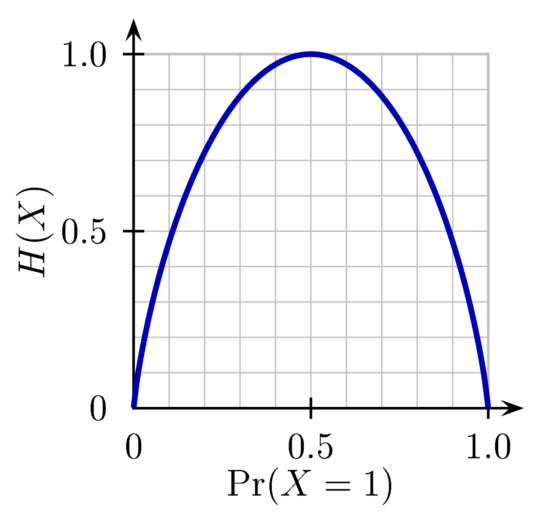
\includegraphics[width=6cm, height=5cm]{Binary_entropy_plot.png}
	\caption{Binary entropy plot from \cite{entropy}}
    \label{entropy}
\end{figure}
Now we want to aggregate information from several  different subsets, e.g. we are splitting on a certain attribute with several different subsets and each of these subsets will have different purity value. When putting them together we want to average their purity values. Since we also want to take into consideration how much splitting we might have left, we weigh each subset according to its size, so the proportion that fall into this subset, namely \( \frac{|S_{V}|}{|S|}\).\\
Our aim is to have items in pure sets. In order to decide whether to split on a feature \( a \) or not, we compute the expected drop in entropy, \textit{Gain(S,a)}, after the split 
\[ Gain(S,a) = H(S) - \sum_{V \in values(a)} \frac{|S_{V}|}{|S|} H(S_V) \]
where \( V \) are the possible values of \( a \), \( S \) is the set of examples \( {X} \) and \( S_{V} \) is the subset where \( X_{a} = V \). This is also known as \textit{mutual information} between attribute \( a \) and class labels of \( S \).

 
\subsubsection{Gini index}
As an alternative to entropy we can use the \textit{Gini index} as a measurement for information gain but we will not go into this any further for now. 

\section{Project Structure}

We implemented the Random Forest as implied above, following the pseudo code in a python implementation. This implementation was handed in as well. The following UML diagram explains the relationship between the classes used in the implementation:


\begin{figure}[!ht]
	\centering
  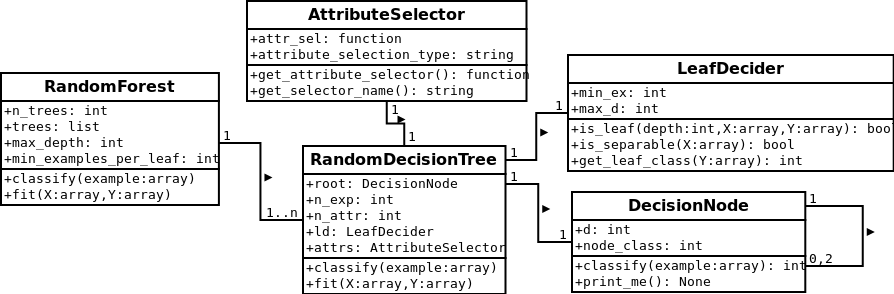
\includegraphics[width=8cm]{Diagram1.png}
	\caption{UML Diagram, best viewed on monitor}
	\label{UML}
\end{figure}

A Random Forest carries a list of Random Decision Trees. The Random Forest's {\tt fit()} method calls the {\tt fit()} method of each Random Decision Tree in its list. The {\tt classify()} method lets the trees in the Random Forest's list democratically vote on the classification.\newline
The Random Decision Tree carries at an instance each of {\tt LeafDecider} and {\tt AttributeSelector}. The tree's {\tt fit()} method constructs a tree as implied above. The tree's {\tt classify()} method propagates the example to be classified through the tree structure.\newline
The {\tt AttributeSelector} contains all the code concerning how a node decides on how to choose the attribute on which it splits the data. A Decision Tree's {\tt AttributeSelector} would pick the "best" splitting value of all possible attributes to split the data on. A Random Decision Tree's {\tt AttributeSelector} would pick the "best" splitting value of \( \log_{2} \)(number of all possible attributes) to split the data on.
The {\tt LeafDecider} is a class that gives all nodes the capability of deciding whether they're a leaf (termination of recursion) or not. The {\tt LeafDecider} checks things such as whether the maximum tree depth is reached, the number of examples in the leaf are still statistically significant, etc.

\section{Results}

\subsection{Evaluation Criteria}
In the following  chapter, the efficacy of the random forest approach is evaluated. We will be applying two classifier metrics to our random forests. We will first define true and false positives, true and false negatives. We will then apply the two metrics, accuracy and confusion matrix to two very different random forests, one with many deep trees and one with few shallow trees.\newline

\subsubsection{Fundamentals}~\\
True Positives: examples that belong to class A and are classified as belonging to A\newline
False Positives: examples that do not belong to class A but are classified as belonging to A\newline
True Negatives: examples that belong to class B and are classified as such\newline
False Negatives: examples that do not belong to class B but are classified as such\newline


\subsubsection{Accuracy}~\\
The accuracy can be understood as the percentage of correctly classified examples. It is defined as: \newline
\\
accuracy(Examples) = (\#TP + \#TN) / (\#Examples)
\\
\\
The table in Fig. \ref{fig0} shows the accuracy of different combinations of the two parameters. The test data consists of almost 1000 pictures of the Simpsons characters, with about 50 pictures per person. The random forest that is built has never seen these pictures before.
\\
The table shows that the accuracy is almost always monotonously increasing in the direction of both the depth and of the number of trees in the forest. %The yellow cells show combinations for which the results are better than 50\%. 
\\
The best result can be found in the entry corresponding to 50 trees with depth 50, with an accuracy of 83\%. This is a convincing result.
\\

\subsubsection{Confusion Matrix}
The confusion matrix is a kind of contingency table. It has two axes, real class and predicted class. It then contrasts all examples by real class to the class predicted by the classifier. 
In our case the confusion matrix has 20 rows and 20 columns. The entry \( (i,j) \) corresponds to the percentage of the character \( i \)'s classification as character \( j \). It is noteworthy that this matrix is not typically symmetrical: mistaking Marge for Homer is not the same as mistaking Homer for Marge.\newline
The accuracy shows positive results. But the quality of information given to us by the confusion matrix is vastly superior to the information of the accuracy alone. In other words, if the forest struggles to classify Marge Simpson, that would not be a good sign because Marge should be easily distinguished thanks to her blue hair \ref{fig6}. If the forest confuses Bart with Lisa, on the other hand, this can be borne, given that they both have spiky hair. 
\\
The matrix is plotted in heat map style, which - instead of the actual percentage - darkens the color of a cell if a cell has a high number and lightens the cell if the number is low. For example, if the cell \( i \times j \)  is white, the character \( i \) has not been classified as character \( j \) at all. 
\\
If the method works well, the diagonal of the confusion matrix should hold the highest values; in other words, the characters should have been classified as themselves most of the time. 
\\
%image 10x20NEW.png
For the combination 50 trees with depth 50 the confusion matrix in Fig. \ref{fig1} looks very much like just described. The diagonal entries are of a dark shade of blue whereas most of the other cells are filled with whitish blue. Homer Simpson seems to have been classified especially well. Possible reasons for that are to be given shortly.
\\
The combination \( 50 \times 50 \) worked well, so now the confusion matrix for the combination \( 15 \times 10 \) is shown in Fig. \ref{fig2}. The accuracy for this combination had just been over 50\%. The actual values of the matrix can be found in Fig. \ref{fig3}.
\\
\begin{figure}[!ht]
	\centering
  
\includegraphics[width=0.2\textwidth]{MargeSimpson.png}
	\caption{Marge Simpson}
	\label{fig6}
\end{figure}
%-----> insert picture 15x10.png
%-----> insert picture 15x10table.png
The matrix shows a distinct diagonal, with some cells much darker than the others. Homer Simpson's diagonal entry is again the darkest and the corresponding value in the matrix is 82\%, i.e. of the Homer Simpson pictures in the test set, the random forest classified 82\% of the pictures as Homer. Other characters who did well were Sideshow Bob who is easily distinguished by his wild reddish hair. The third best candidate is Ned Flanders, who is presumably recognizable by his green sweater. 
\begin{figure}
\subfloat[Homer Simpson\label{fig:Homer}]
  {
\includegraphics[width=.3\linewidth]{Homer}}\hfill
\subfloat[Sideshow Bob\label{fig:sideshowbob}]
  {
\includegraphics[width=.3\linewidth]{sideshowbob}}\hfill
\subfloat[Ned Flanders\label{fig:nedflanders}]
  {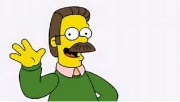
\includegraphics[width=.3\linewidth]{NedF}}
\caption{The characters who were the easiest to classify correctly}
\end{figure}
\\
The character who did worst was Nelson Muntz, who was correctly classified only 2\% of the time. As there are 50 pictures per character in the test set, only one picture of Nelson was classified as Nelson by the random forest. The other two worst characters are Lenny Leonard and Mayor Quimby, with 6 and 16\% respectively. 
\\
\begin{figure}
\subfloat[Nelson Muntz\label{fig:NelsonM}]
  {
\includegraphics[width=.3\linewidth]{NelsonM}}\hfill
\subfloat[Lenny Leonard\label{fig:lennyL}]
  {
\includegraphics[width=.3\linewidth]{LennyL}}\hfill
\subfloat[Mayor Quimby\label{fig:mayorQ}]
  {
\includegraphics[width=.3\linewidth]{mayorQ}}
\caption{The characters who were the hardest to classify correctly}
\end{figure}
Out of the 20 characters, 11 characters were classified as themselves more than 50\% of the time, which is well satisfactory. 
\\
The nice thing about the confusion matrix, though, is that it is easy to see which characters the Simpsons have been confused with most of the time, i.e. what are the highest numbers in each row aside from the diagonal entry. It can be observed, for example, that Nelson Muntz who did badly on the diagonal has been classified as Homer Simpson 40\% of the time. Another high value can be found in the entry corresponding to Lenny Leonard and Ned Flanders, stating that Lenny Leonard was classified as Ned Flanders 34\% of the time. 
\\
As humans, the reason for this could easily be explained by the characters' appearances. Lenny Leonard is brown-haired and wears a green sweater, just like Ned Flanders. Nelson Muntz, though, has seemingly nothing in common with Homer Simpson. So why is he classified as Homer so often?
\\
Again, an unscientific explanation would be that, since Homer is the main character but still a very ordinary person in the show, he was given the most ordinary Simpsons features. It is easy to see that his son Bart, for example, has the same face except for Homer's beard and Bart's hair. So one possible reason that all of the characters were confused with Homer so often might that he shares common face or clothes features with all of the other characters. 
\\
The mathematical reason can be found looking at the data structure of the training set, though. The training set consists of folders of pictures for each character, as was downloaded from Kaggle. But the folders are not equally big, in other words, in Homer's folder there are much more pictures than in Nelson's, around 2300 pictures to 220 to be exact. So the decision tree, if it does not have a big enough depth, learns much more about Homer's features and concentrates more on classifying Homer correctly than it cares about Nelson. Of course it would have been much more appropriate from a machine learning point of view to have equally sized folders. Another way would have been to put weights on the characters to make up for any difference in number of pictures in the training set.
\\
This also explains why Ned Flanders is classified correctly most of the times:  in the training set, his folder contains 1500 pictures. 
\\
To take a look at Marge Simpson: She has been classified correctly 68\% of the time, so she is in the top seven. She was classified as Chief Wiggun 4\% of the time, which is a surprisingly small value, given that they both show a lot of blue color. 
\\
%-----> insert picture 15x5.png
Looking at Fig. \ref{fig4}, a very interesting thing to finish with is the heat map for the combination 15 trees with depth 5. The accuracy is not as good now: the diagonal does not seem as dark as for the other combination before. But it seems that the most prominent features of the characters are more important when there is less depth in the tree: Homer is still classified the best at 80\%, possibly due to the reason just explained, but now Marge Simpson, Sideshow Bob and Chief Wiggun, the most easily recognizable characters, lead the way with 76, 59 and 42\% correct classifications. This means that the decision trees, when constrained in their depth, look for the broader features to classify the characters, whereas if the tree is allowed to grow longer, other details become more important. This can also be seen in the corresponding table in Fig. \ref{fig45}.
\\
Interestingly enough, the same effect does not appear when the size of the forest is reduced instead of the depth: the heat map becomes more diverse and it is harder to distinguish the diagonal. It is harder to classify the characters as themselves and even Homer is only recognized 42\% of the time. 
\subsection{Summary} 
The random forest method yields convincing results if the number of trees in the forest and their depths is high enough. It is quite dependent on the training set, though, as can be seen looking at Homer Simpson: he does well because his folder in the training sets contains the most pictures. The characters with the highest accuracy are either main characters - meaning they have many pictures in the training set's folder - or have significant features such as Sideshow Bob. If you reduce the depth of the tree, the significant features are more important and suddenly characters like Marge and Chief Wigguns do well. 
\\
\section{Outlook}
There are other tree methods that yield even better results than the random forests. There are the so-called \textit{Extra trees} \cite{extratrees} which are a highly randomized version of the random forest. They differ from the random forest in two important facts: the splitting of the nodes is completely random and the whole training sample is used for creating the trees. In practice, the extra trees performed better than the random forest for the Simpson test data set. For a combination of enough trees with enough depth, they reached a 100\% accuracy for the test set.
\\
\newpage
\newpage
\appendix
\section{Appendix}
\textbf{The following pictures are best viewed on a monitor! 
}\begin{figure}[!ht]
	\centering
  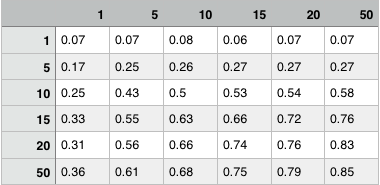
\includegraphics[width=0.5\textwidth]{table1.png}
	\caption{Accuracy for combinations of number of trees and depth of the trees. The rows correspond to the depth, the columns to the number of trees. The accuracy in most of the time increasing in the direction of the depth of the trees and the number of trees.}
	\label{fig0}
\end{figure}
\begin{figure}[!hb]
  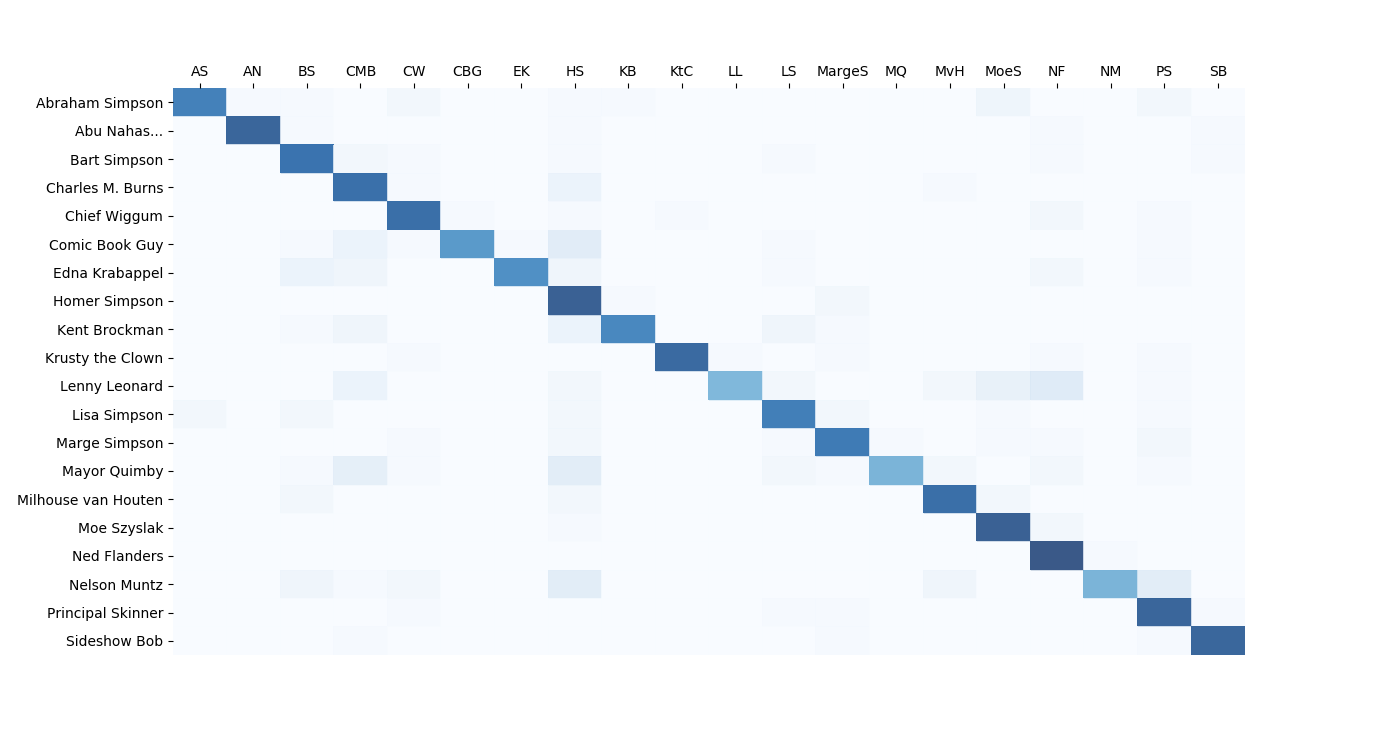
\includegraphics[width=0.5\textwidth]{50x50.png}
	\caption{Confusion matrix heatmap for the combination 50 trees of depth 50. The diagonal is very distinct and shows that most of the characters are classified as themselves with a high percentage.}
	\label{fig1}
\end{figure}
\newpage
\begin{figure}[!ht]
	\centering
  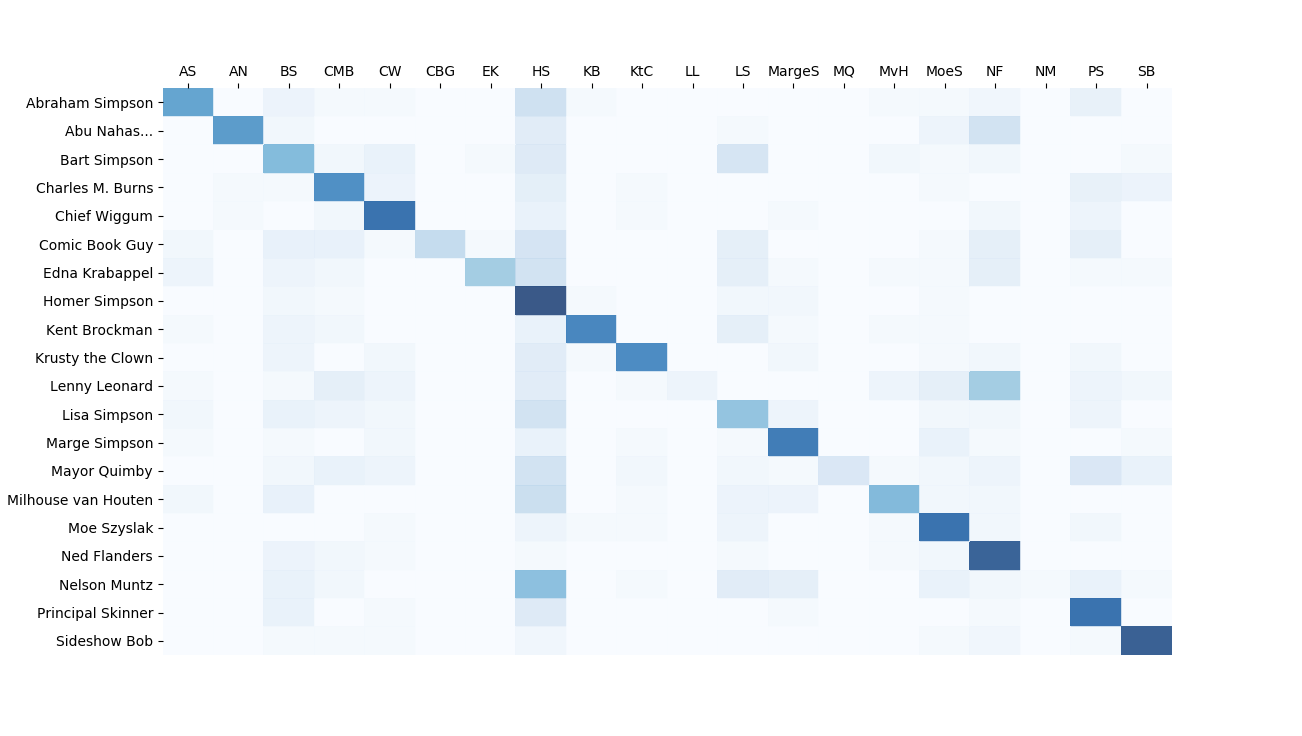
\includegraphics[width=0.5\textwidth]{15x10.png}
	\caption{Confusion matrix heatmap for the combination 15 trees of depth 10. The diagonal is not as distinct as in the \( 50 \times 50 \) case but it is still recognizable.}
	\label{fig2}
\end{figure}
\begin{figure}[!hb]
	\centering
  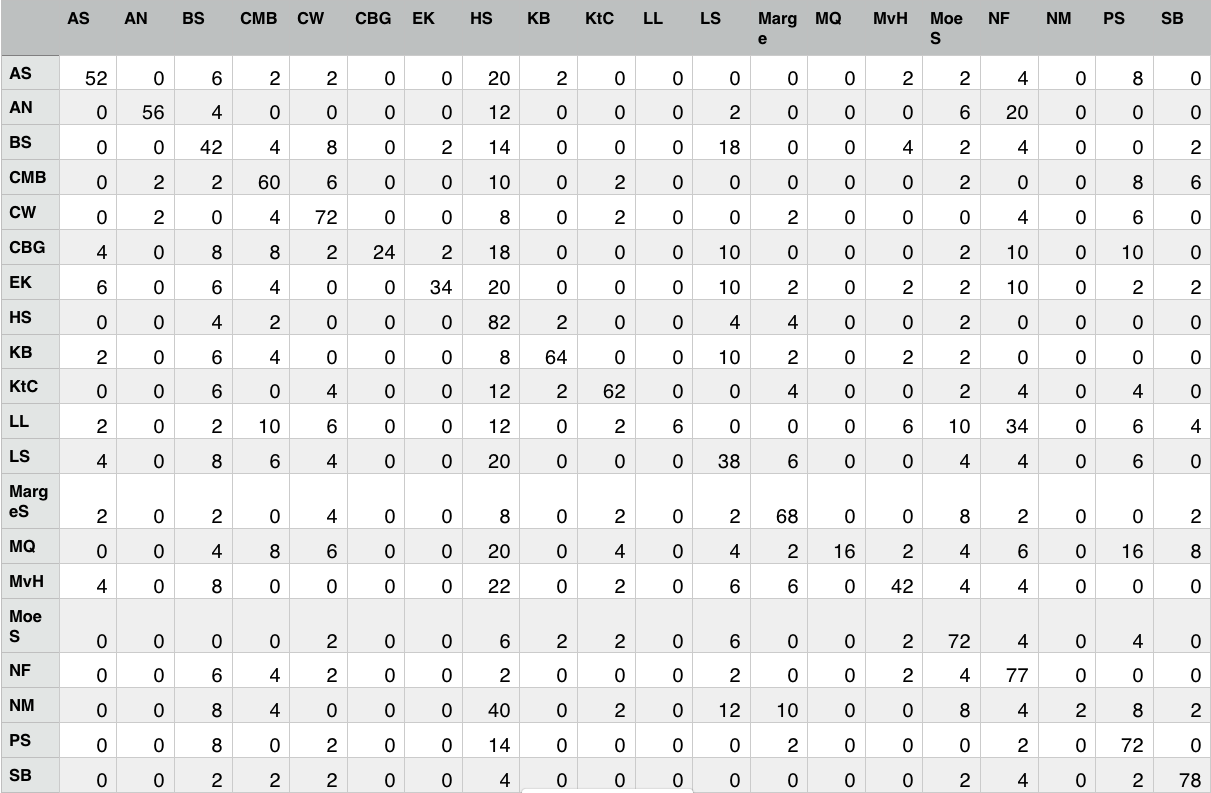
\includegraphics[width=0.4\textwidth]{15x10table.png}
	\caption{Confusion matrix for the combination 15 trees of depth 10.}
	\label{fig3}
\end{figure}
\newpage
\begin{figure}[!ht]
	\centering
  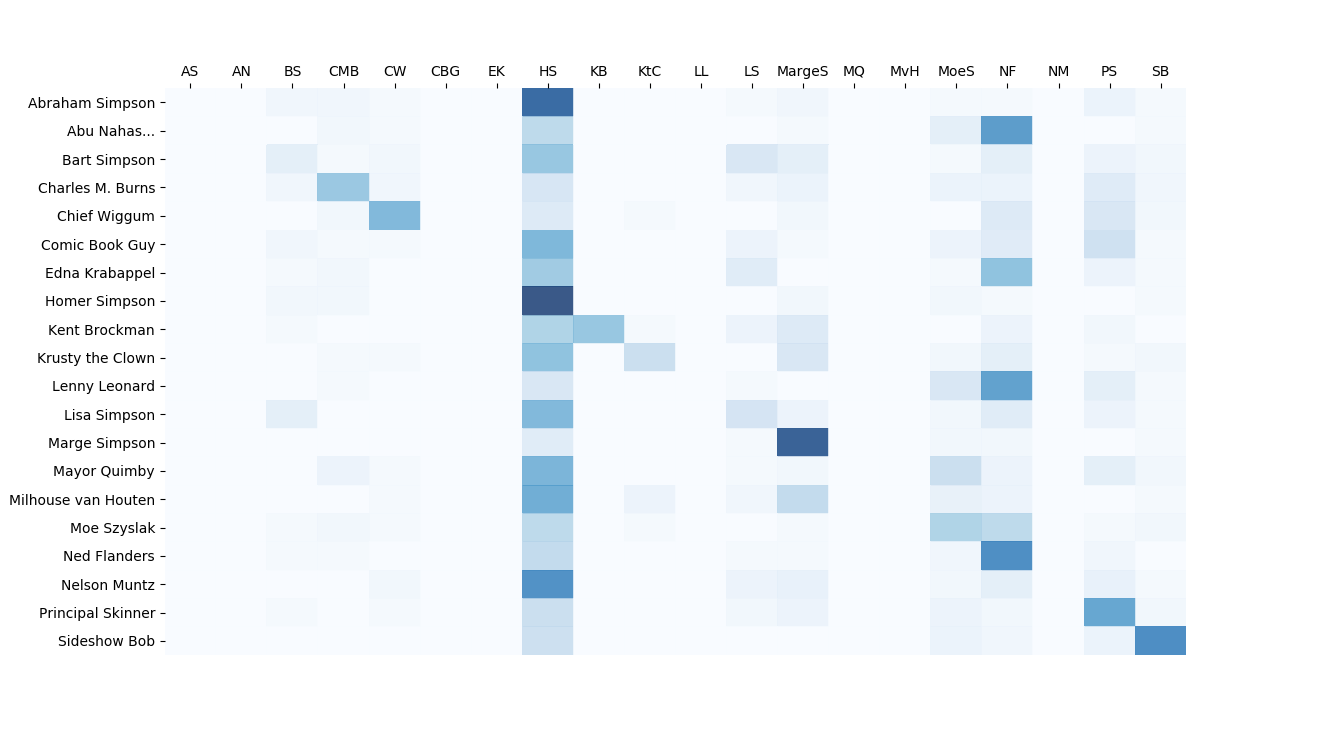
\includegraphics[width=0.4\textwidth]{15x5.png}
	\caption{Confusion matrix heatmap for the combination 10 trees of depth 5. The diagonal is not easily distinguishable. Single cells on the diagonal show a deeper color and those cells correspond to characters with prominent features such as Marge.}
	\label{fig4}
\end{figure}
\begin{figure}[!ht]
	\centering
  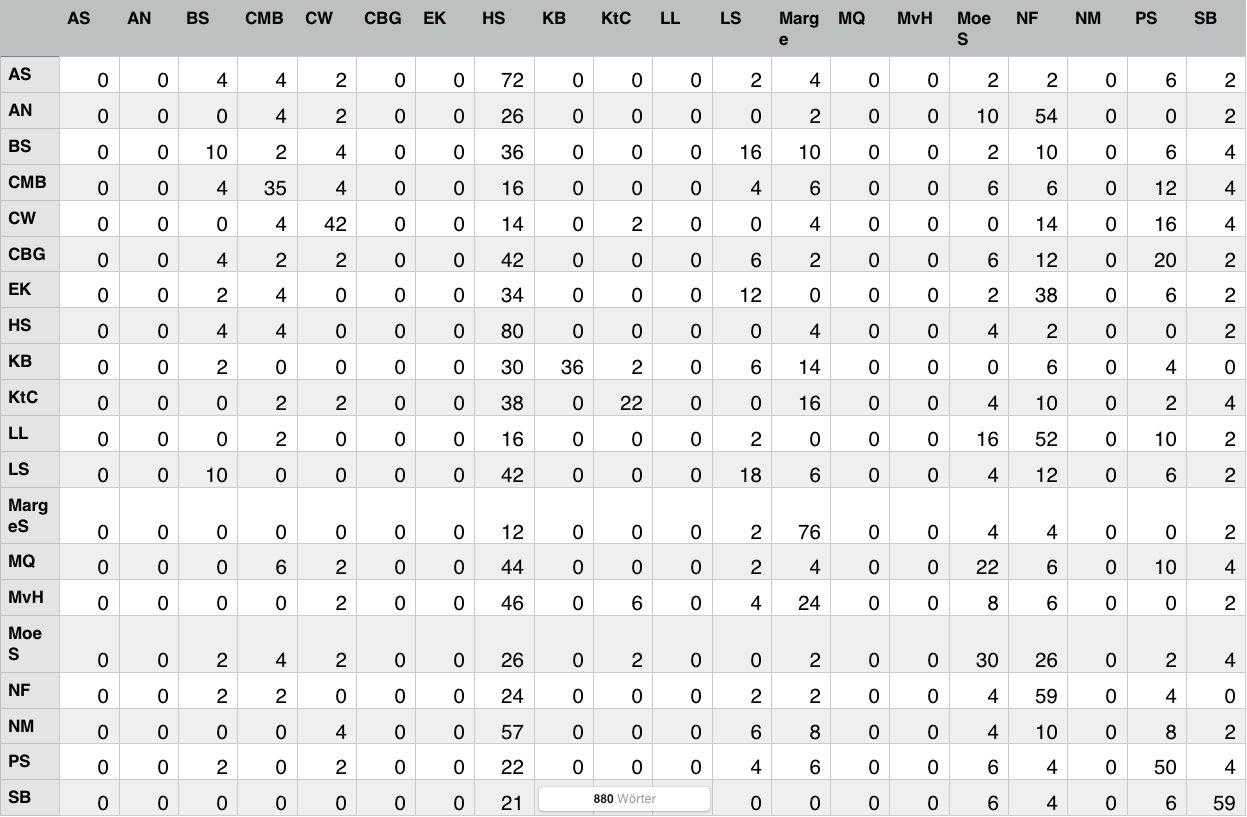
\includegraphics[width=0.4\textwidth]{15x5table.png}
	\caption{Confusion matrix for the combination 10 trees of depth 5. The diagonal is not easily distinguishable. Single cells on the diagonal show a deeper color and those cells correspond to characters with prominent features such as Marge.}
	\label{fig45}
\end{figure}


% Now we need a bibliography:
\begin{thebibliography}{5}

	%Each item starts with a \bibitem{reference} command and the details thereafter.
    \bibitem{pseudocode}
    http://www.otnira.com/2013/03/25/c4-5/, 18/07/2017
    \bibitem{extratrees}
    http://www.montefiore.ulg.ac.be/\~ernst/uploads/news/id63/extremely-randomized-trees.pdf, 18/07/2017
	\bibitem{Histogram of Oriented Gradients}
    Histograms of Oriented Gradients for Human Detection, by N. Dalal, B. 		Triggs, in CVPR '05
    \bibitem{Random Forests}
    Random Decision Forests, by Tim K. Ho, 1995 in Proceedings of the 3rd International Conference on Document Analysis and Recognition, Montreal, QC
    \bibitem{decisiontree}
    http://cloudmark.github.io/images/kotlin/ID3.png, 18/07/2017
    \bibitem{entropy} 
    				https://upload.wikimedia.org/wikipedia/commons/c/c9/Binary\_entropy\_plot.png, 18/07/2017
    
\end{thebibliography}

% Your document ends here!
\end{document}
